\chapter{Real-Life Measurements}

\section{Basic Isotropic Needle Probe Measurements}

The device

The hardware

\begin{figure}[h]
\centering
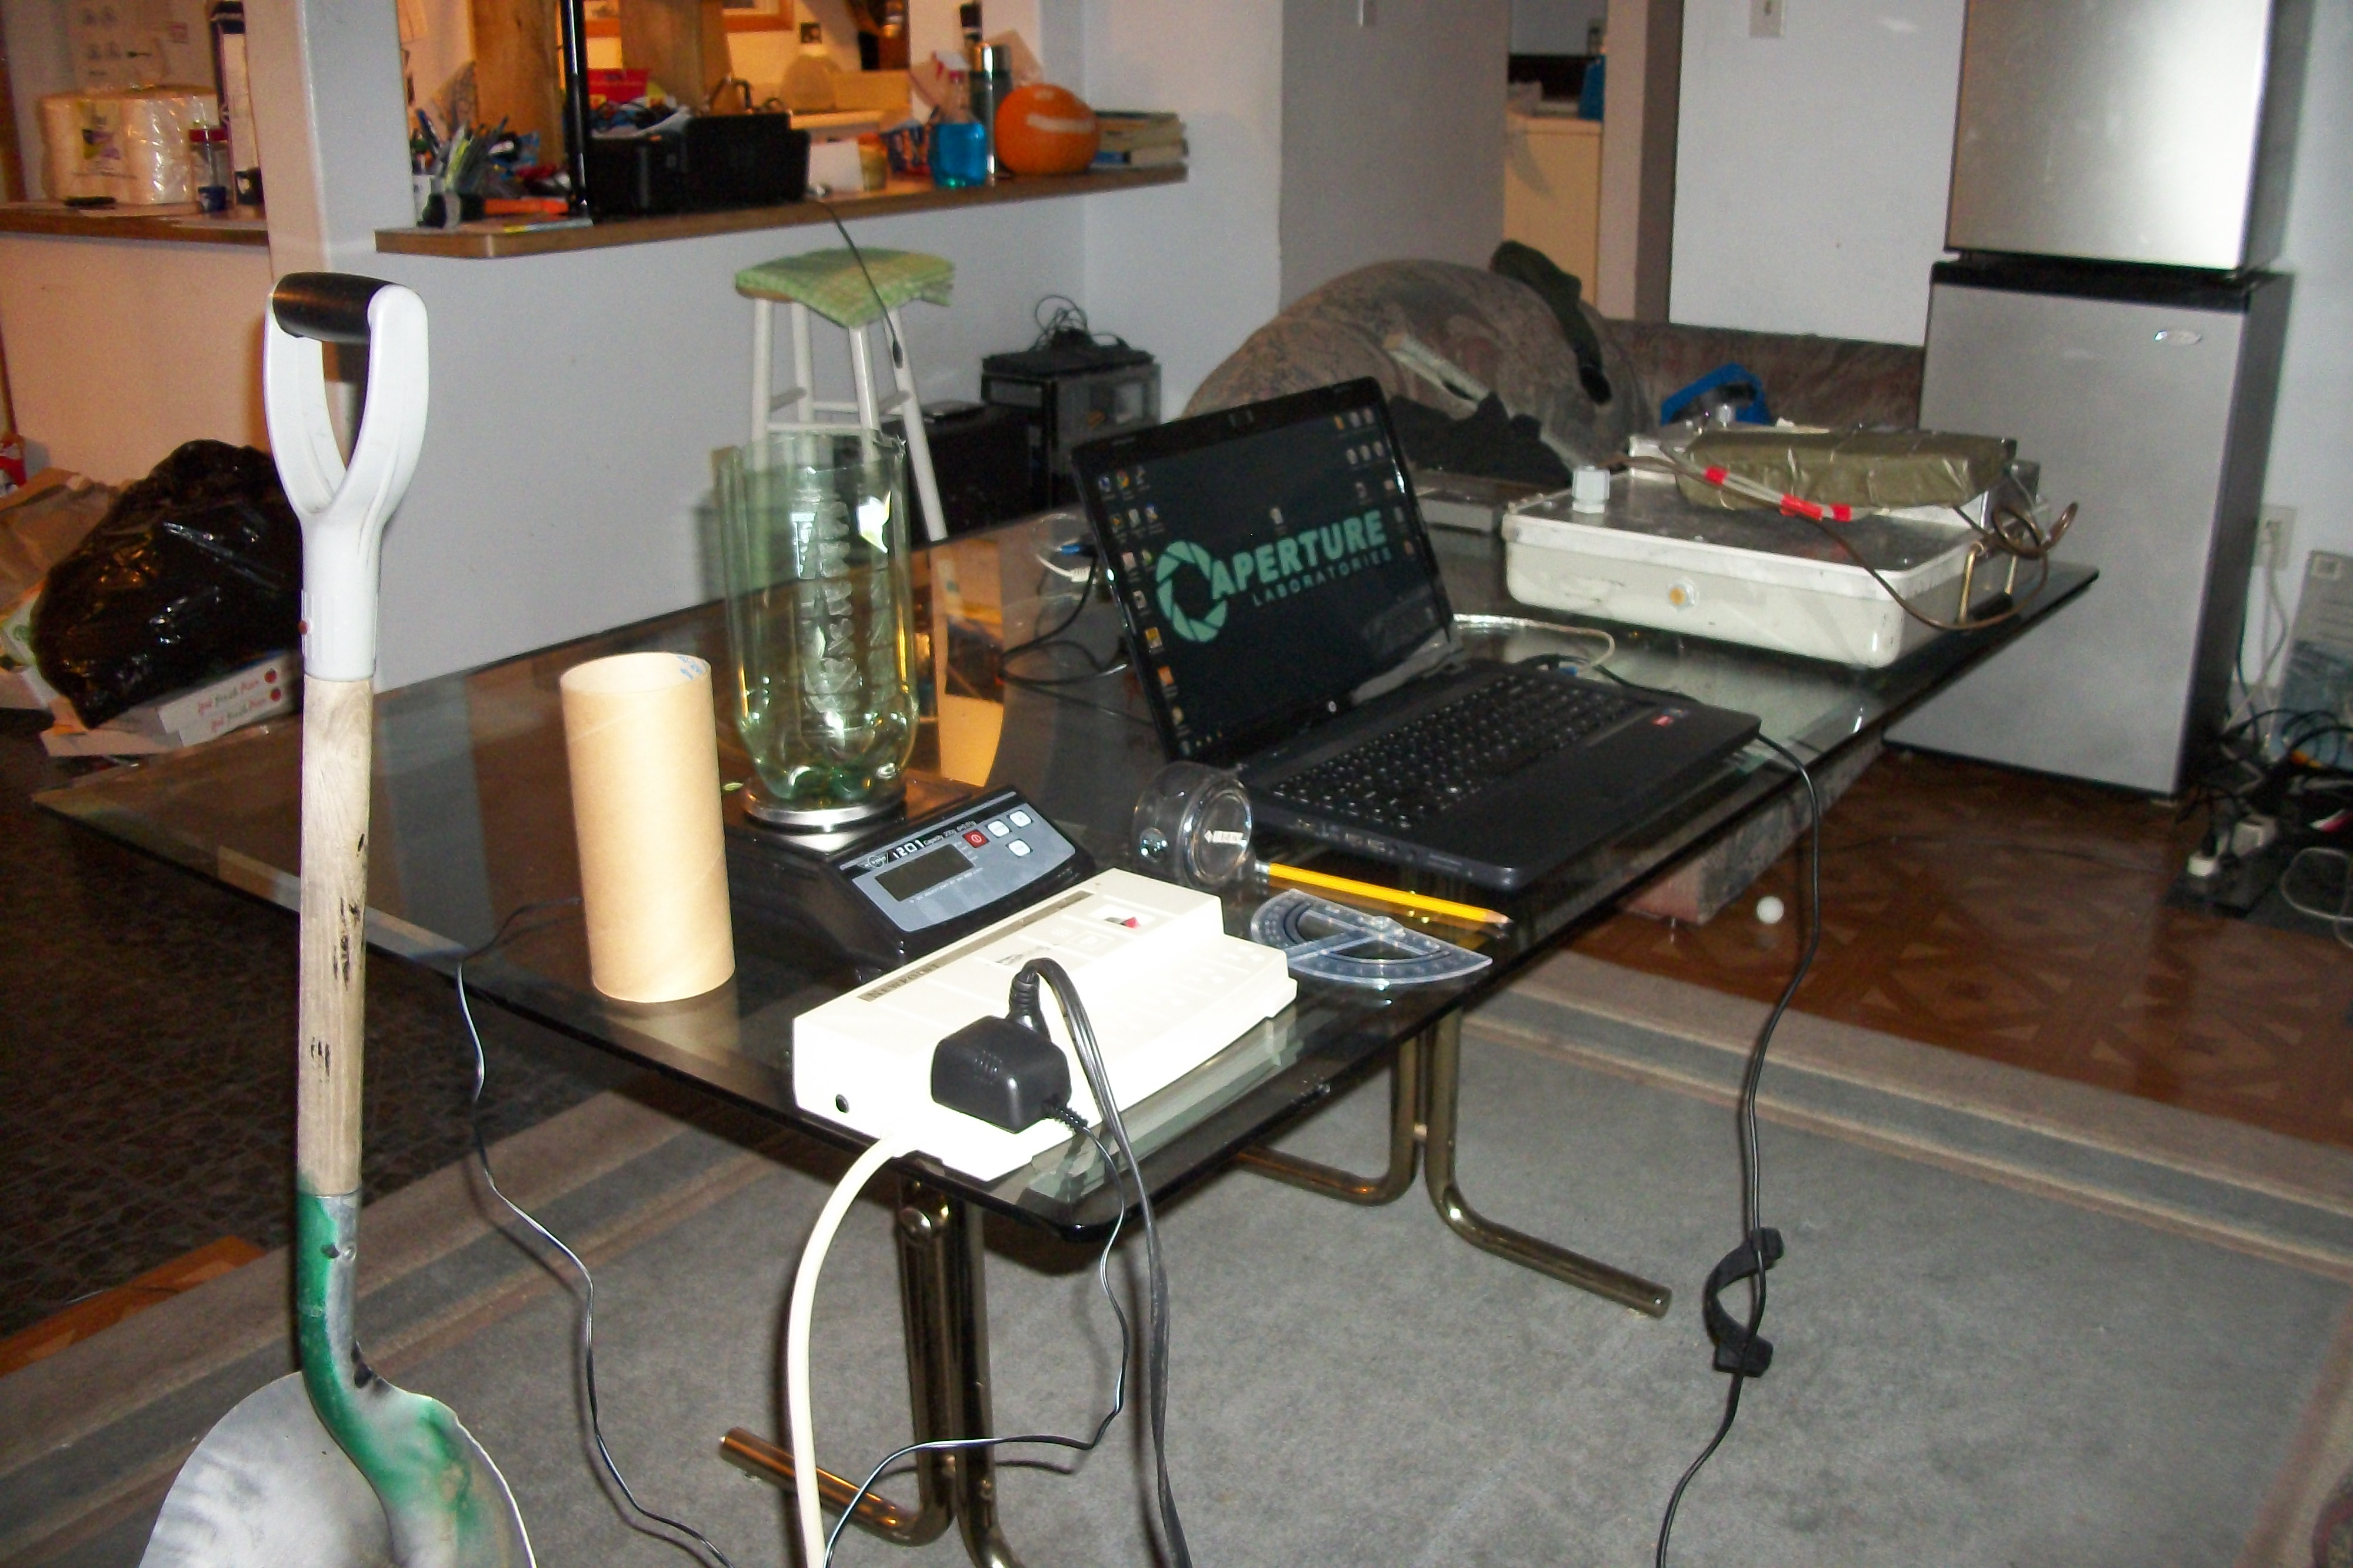
\includegraphics[width=0.8\textwidth]{fig/equipment.jpg}
\label{fig:equipment}
\caption{Equipment used to measure snow thermal conductivity.}
\end{figure}

\begin{figure}[h]
\centering
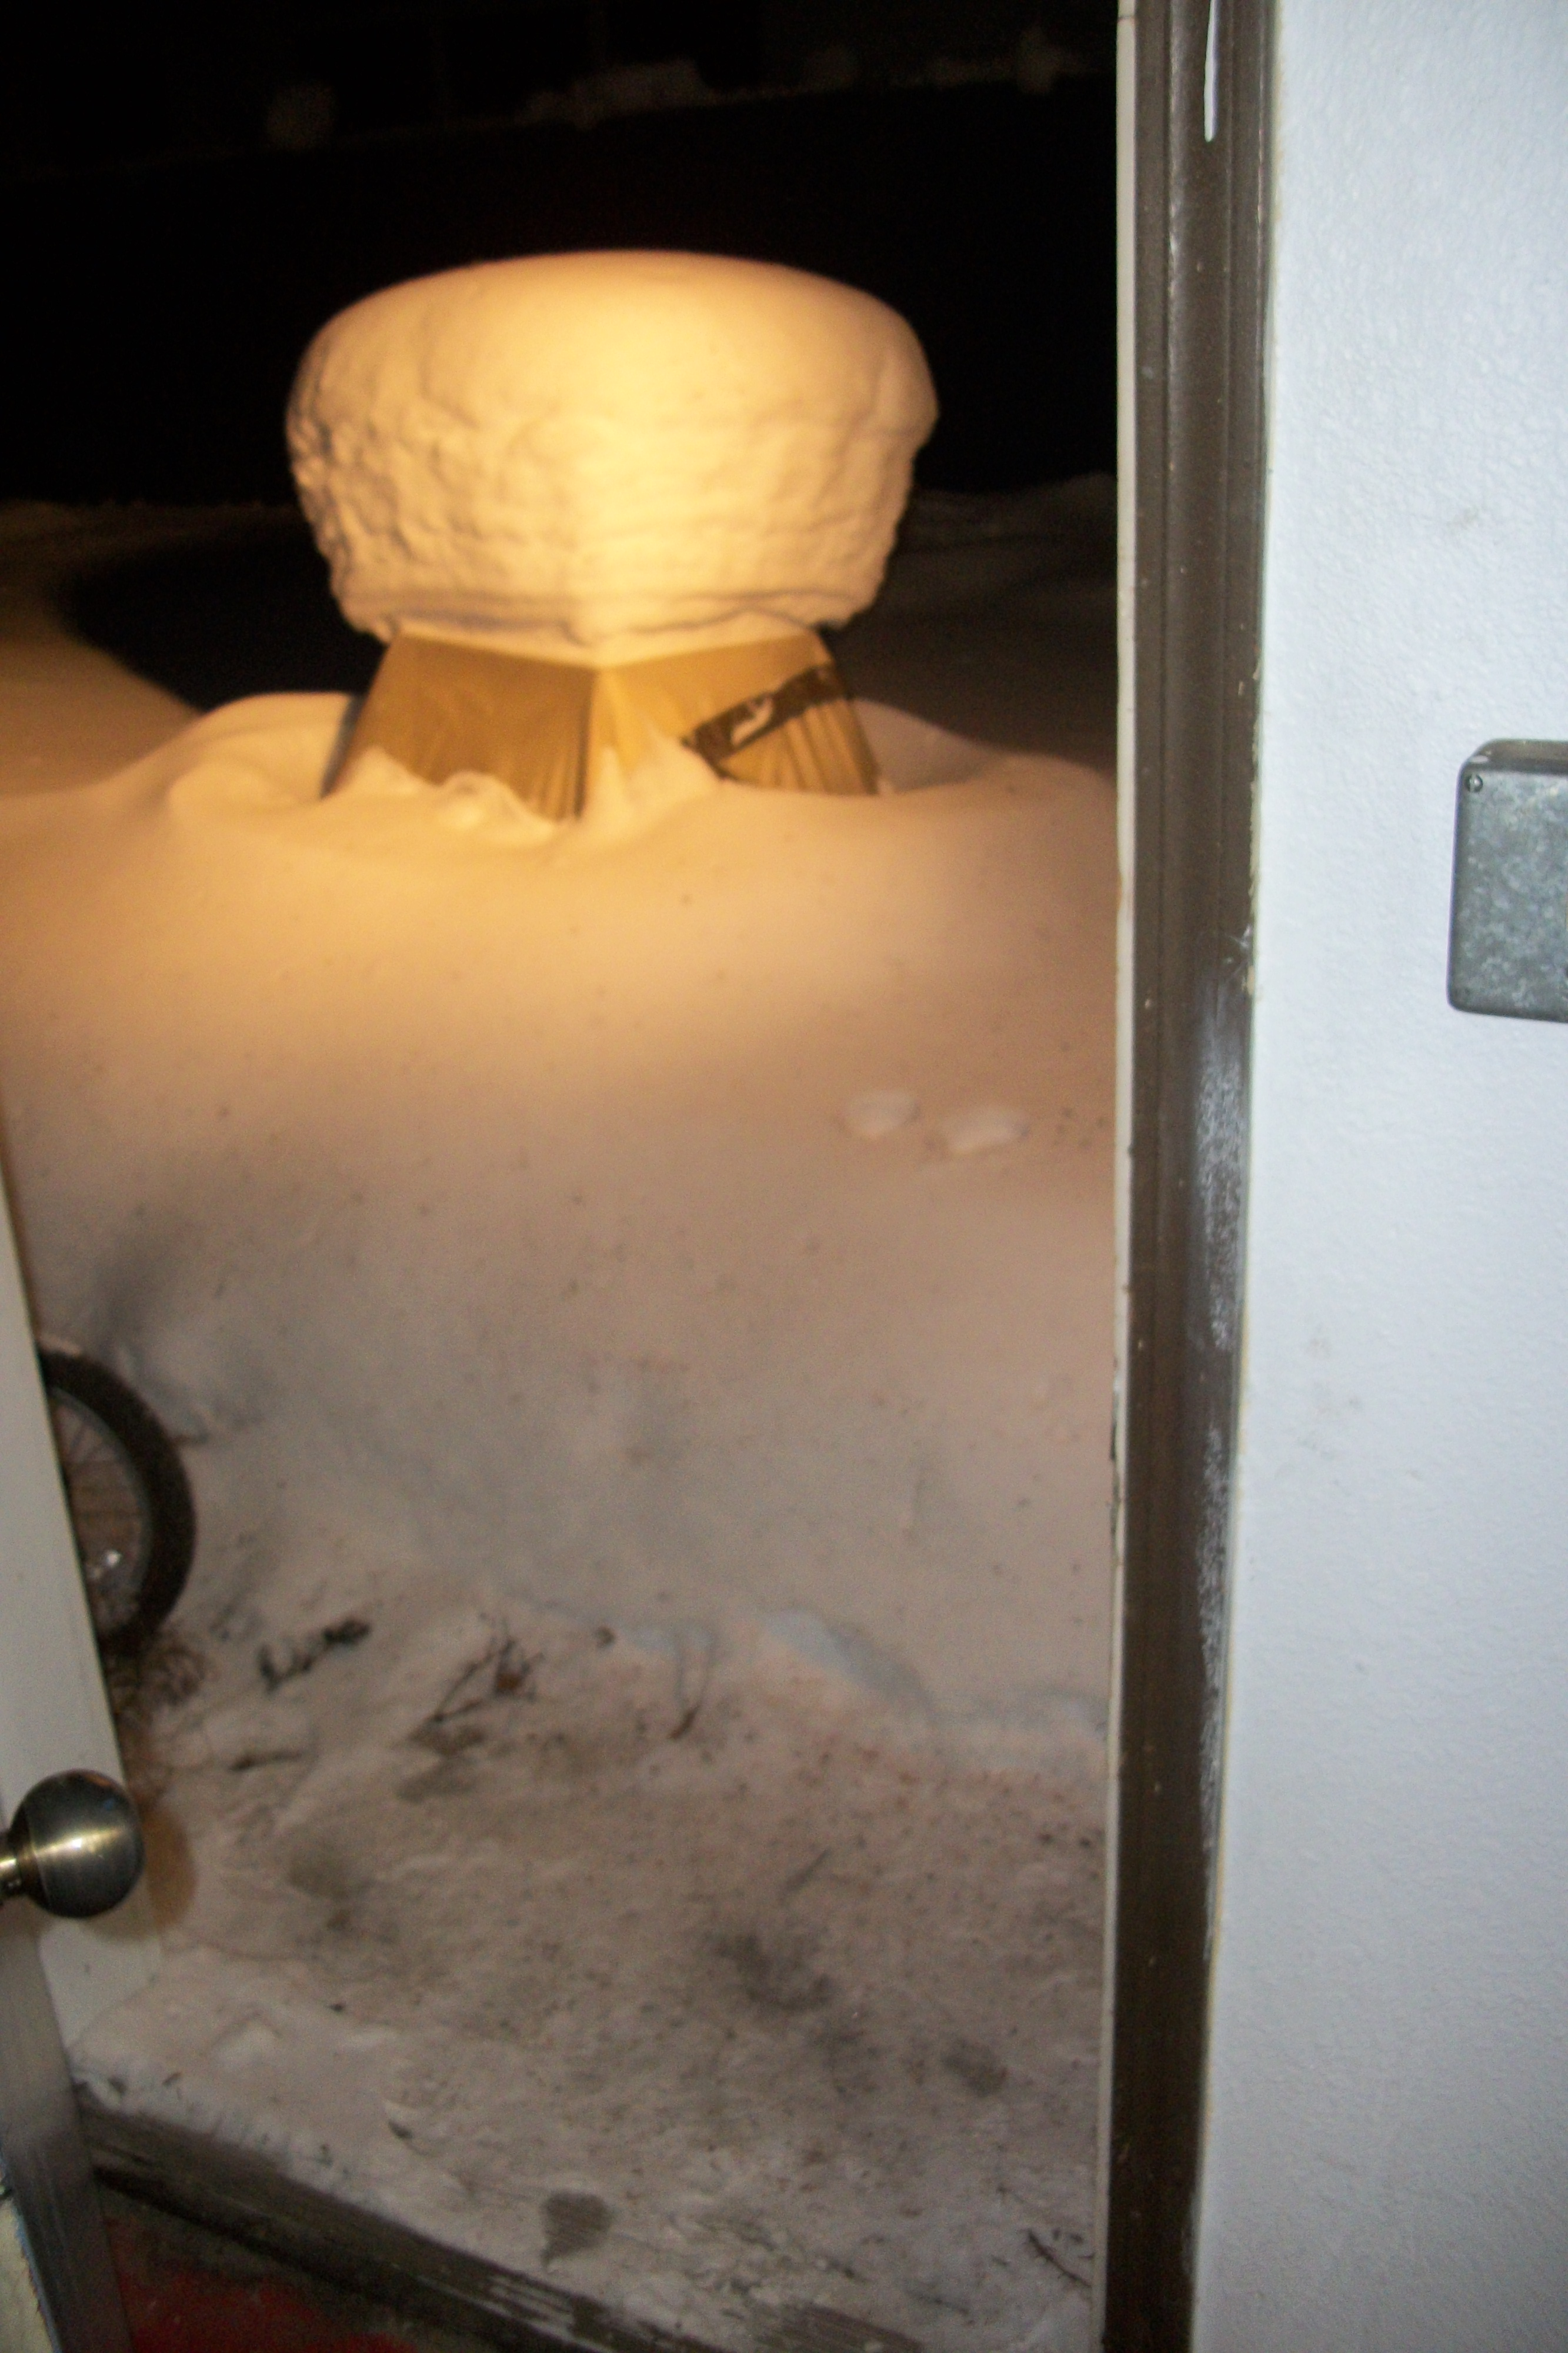
\includegraphics[width=0.4\textwidth]{fig/insitu_location.jpg}
\label{fig:insitu_location}
\caption{The location for in-situ tests.}
\end{figure}

\begin{figure}[h]
\centering
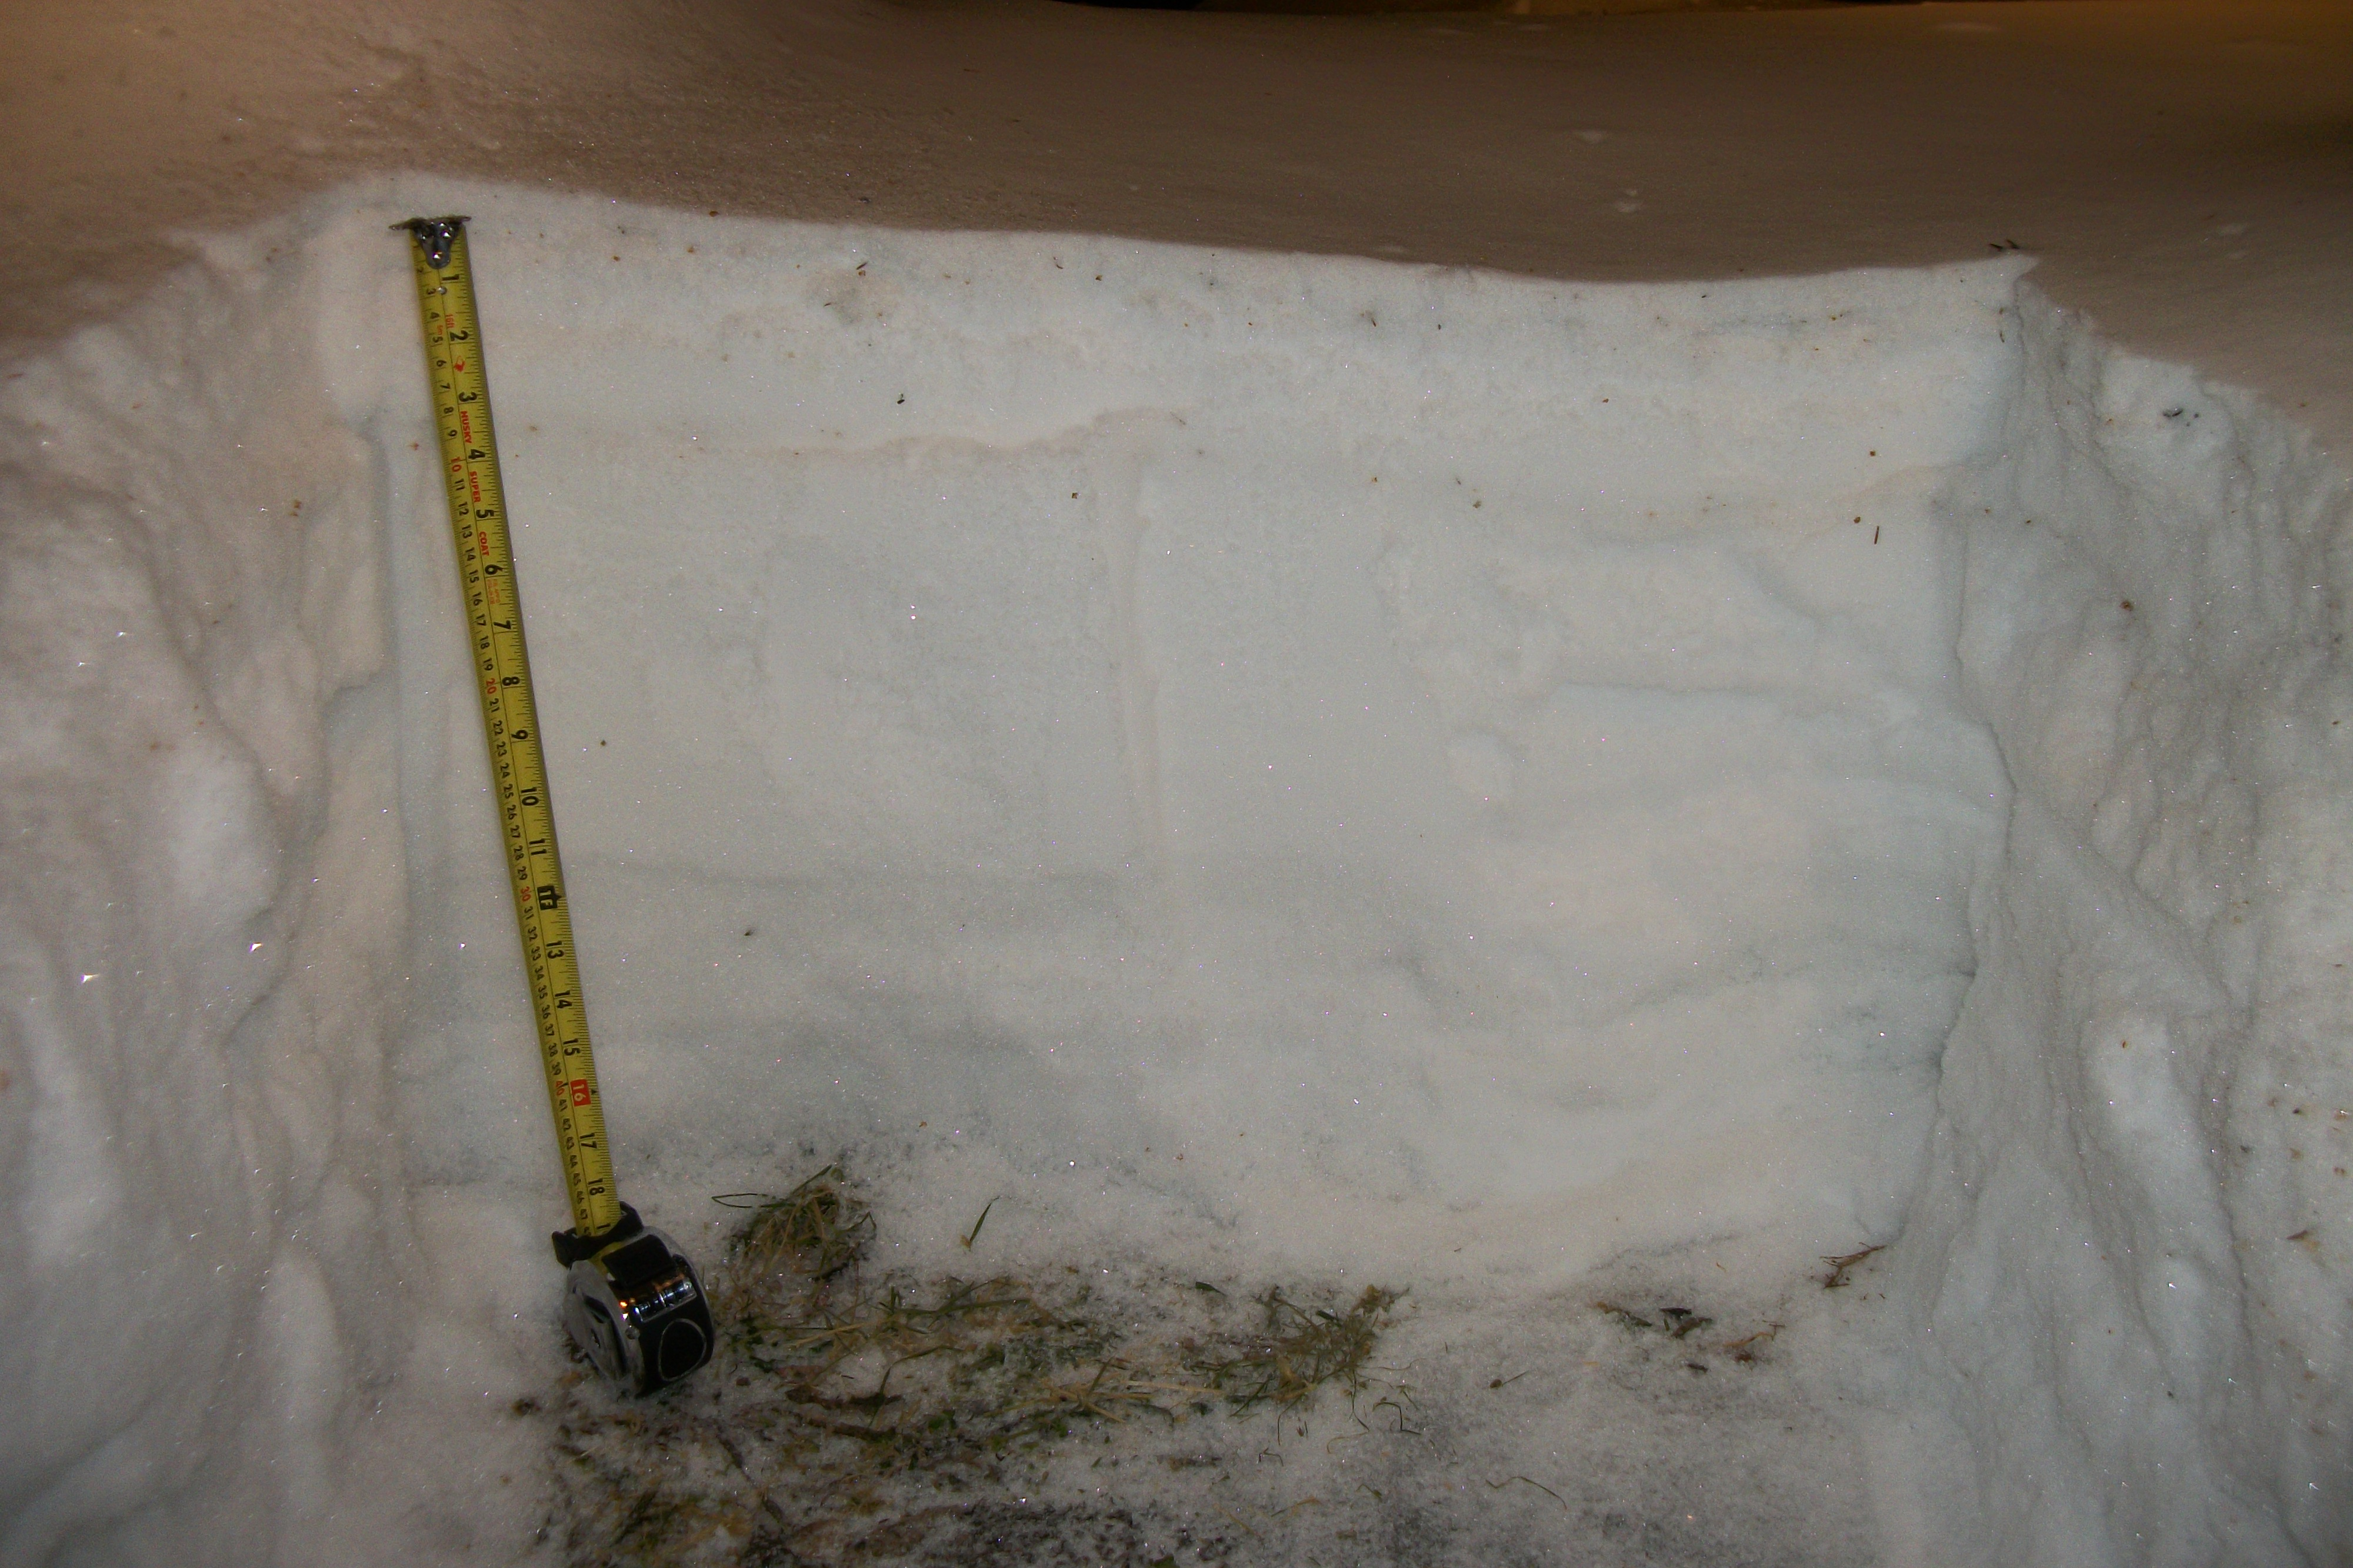
\includegraphics[width=0.8\textwidth]{fig/snowpack.jpg}
\label{fig:snowpack}
\caption{A close-up shot of tested snowpack.}
\end{figure}

\begin{figure}[h]
\centering
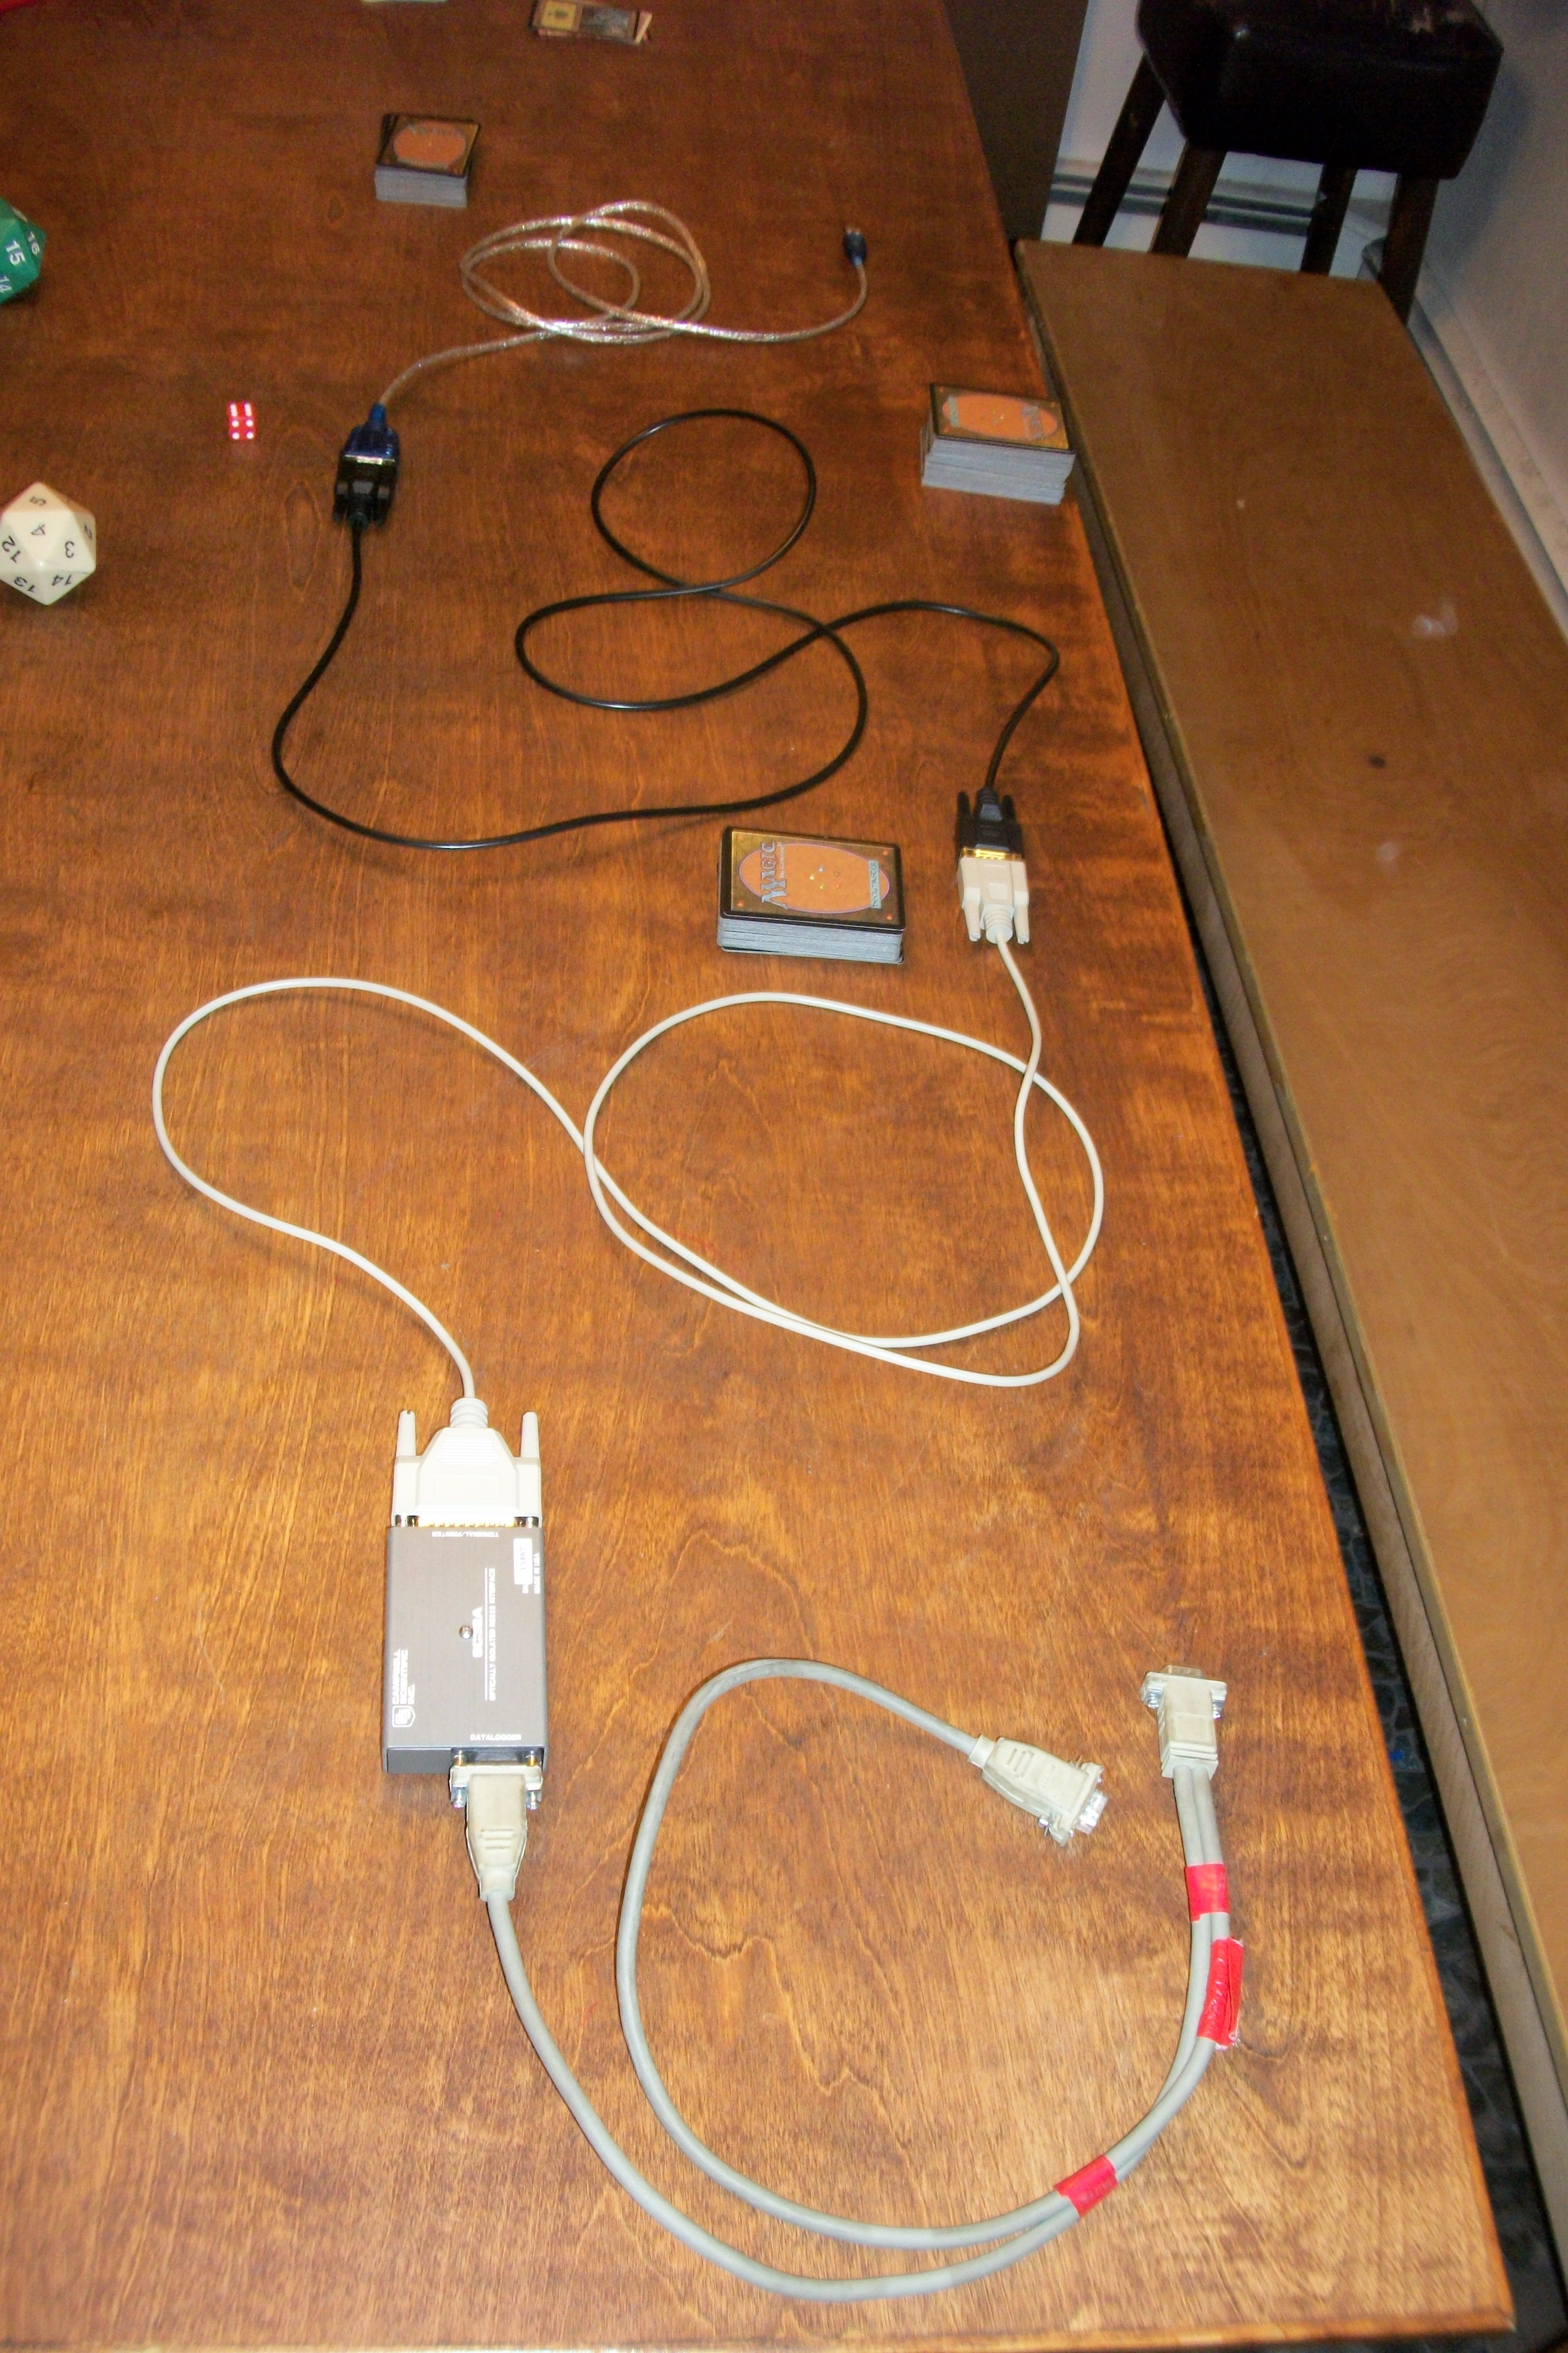
\includegraphics[width=0.6\textwidth]{fig/cable.jpg}
\label{fig:cable}
\caption{The cables used to communicate with the datalogger.}
\end{figure}

The data

The analysis

\section{Benchtop Tests with Glycerine}

The box

\section{Anisotropic Glycerine}

Layers

low K layer

high K layer

tests of both materials alone

\section{Snow Measurements}

technique
